\documentclass{article}

\usepackage[a4paper, left=1.5cm, right=1.5cm, top=2cm, bottom=2cm]{geometry}
\usepackage{../components/components} % <-- ton fichier .sty, avec toutes tes définitions

\usepackage{fancyhdr}

% Configuration des en-têtes et pieds de page
\pagestyle{fancy}
\fancyhf{} % reset tout

\fancyhead[L]{DL Math-Info}
\fancyhead[C]{Modèle type de document}
\fancyhead[R]{2025-2026}

\fancyfoot[L]{Ewen Rodrigues de Oliveira}
\fancyfoot[R]{\thepage}

\begin{document}

\docTitle{Modèle type de document}

\section{Page Composants}

\subsection{Définitions et Théorèmes}

Voici un exemple d’utilisation de tes composants :

\definition{Soit une suite \((u_n)_{n \in \mathbb{N}}\) quelconque. On dit que \((u_n)\) est décroissante si pour tout \(n \in \mathbb{N}\), on a \(u_n \geq u_{n+1}\).}

\theorem{Théorème}{Pythagore}{true}{
    Dans un triangle rectangle, le carré de l'hypoténuse est égal à la somme des carrés des deux autres côtés.
}

\vspace{1em}
\subsection{Carreaux}
\vspace{1em}

\noindent\textbf{Preuve :} \\[0.5em]
\hspace{\parindent}\carreaux{5}

\vspace{1em}
\subsection{Remarques de cours}
\vspace{1em}

\remark{Lorem ipsum dolor it amet, consectetur adipiscing elit.}
\attention{Lorem ipsum dolor sit amet, consectetur adipiscing elit.}
\illustration{Lorem ipsum dolor sit amet, consectetur adipiscing elit.}
\example{Lorem ipsum dolor sit amet, consectetur adipiscing elit.}
\vocabulary{Lorem ipsum dolor sit amet, consectetur adipiscing elit.}
\training{Lorem ipsum dolor sit amet, consectetur adipiscing elit.}

\newpage

\vspace{1em}
\subsection{Autres commandes utiles}
\vspace{1em}

\textbf{1. Code :}
\begin{lstlisting}[language=Python]
def seuil(n):                  # Déclaration de la fonction à un argument
    for i in range(len(n)):    # Parcours de la liste n
        if n[i] < 0:           
            return i           # Retourne l'indice du premier élément négatif
    return len(n)              # Retourne la longueur de la liste si aucun élément n'est négatif
\end{lstlisting}

\textbf{2. Matrices :}
\[
    \begin{pmatrix}
        a & b & c \\
        d & e & f
    \end{pmatrix}
\]
\[
    \begin{bmatrix}
        a & b & c \\
        d & e & f
    \end{bmatrix}
\]
\[
    \begin{vmatrix}
        a & b & c \\
        d & e & f
    \end{vmatrix}
\]

% Matrices avec second membre

\[
    \begin{pmatrix}
        a & b & c & | & g \\
        d & e & f & | & h
    \end{pmatrix}
\]

\[
    \left(
    \begin{array}{cc|c}
            2 & 1 & 5 \\
            1 & 3 & 7
        \end{array}
    \right)
\]

\textbf{3. Graphiques :}

On a le graphique suivant :
\begin{center}
    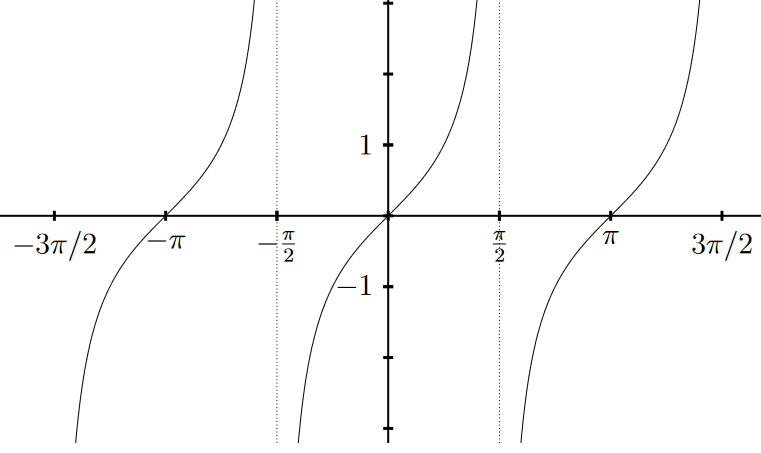
\includegraphics[width=0.5\textwidth]{../images/tan.png}
    \captionof{figure}{Graphe de la fonction tangente sur \([- \pi/2, \pi/2]\).}
\end{center}

Ou bien: \newline
\captionsetup{justification=raggedright, singlelinecheck=false}
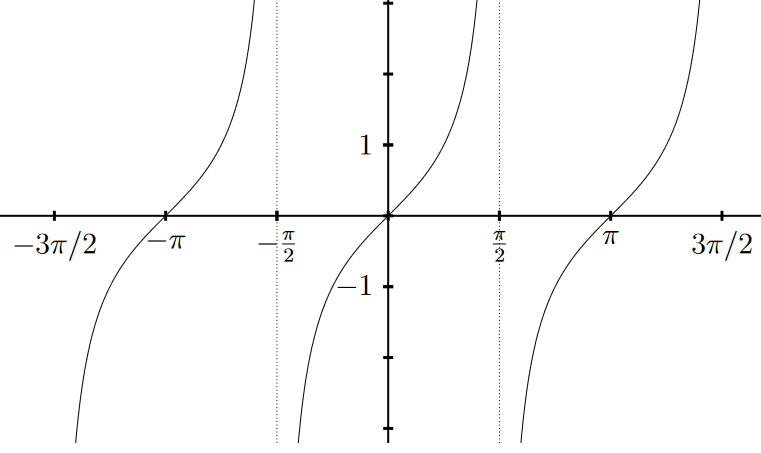
\includegraphics[width=0.5\textwidth]{../images/tan.png}
\captionof{figure}{Graphe de la fonction tangente sur \([- \pi/2, \pi/2]\).}

\end{document}
